\section{Semantic Knowledge Learning}
\label{sec:scene-ridge-climbing}
The results generated by \gls{hdp} are several clusters of visual words, however, without any semantic meaning.
This section describes some post-processing steps for extracting higher-level semantic knowledge of the camera scene.

\subsection{Robust Ridge Climbing}
    Just by looking at the topics in \ref{fig:scene-topics}, we could roughly infer how the vehicles move in the video. 
    More importantly, the extent of the high-density grids gives useful insights into the size and moving region of the tracked objects. 
    Let $\phi$ be a multinomial distribution of a topic learned by \gls{hdp}. For any grid $i$, it has $D$ values, corresponding to $D$ evenly quantized directions, written as $\bm{\phi}_i= [\phi_i^{1}, \phi_i^{2}, \dots, \phi_i^{D}]$.
    We define two terms:
    $d^*_i = \argmax_{d}(\phi_i^{d})$ is the \emph{dominate direction} of grid $i$, which has the maximal value of distribution among all directions.
    We also define a terms summing over all the directions of each grid $\varphi_{i} = \sum_{d=1}^{D}{\phi_i^{d}}$.
    Figure \ref{subfig:scene-grid-dist} shows an example of the distribution of a certain topic on a grid, where the radius of each sector indicates the value of $\phi_i^{d}$. 
    In this topic, the grid has the highest $\phi_i^d$ with $d=1$, indicating that it will be most likely to move along this direction. 
    \ref{fig:scene-ridge-clibming} gives a 3D visualization of the first topic in \ref{fig:scene-topics}, where the height at each grid is $\varphi_{i}$. 
    Overall they form a mountain-like surface. We aim to learn the shape and extent by extending the ridge climbing method in \cite{zhao2013counting}. 
    The idea of this method is to start from a high-density grid, make one step iteratively until reaching the image boundary or the low-density area. 
    The steps move along the desired direction and follow the shape of the topic distribution. 
    For the purpose of consistency, all the following examples will be on the first topic in \ref{fig:scene-topics}.
    % Due to the different views of the videos, some topics may expand a wide area, resulting ridge, not in the center of the high-density area. Accordingly, we improve this method by getting multiple ridges and then shrink them into a more confident center line.
    \begin{figure}
\centering
    \begin{subfigure}{0.48\linewidth}
        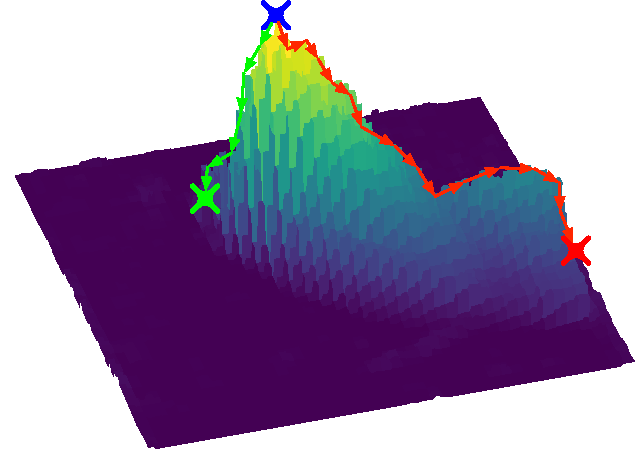
\includegraphics[width=\linewidth]{./img/scene_learning/ridge_climbing.pdf}
        \subcaption{}
        \label{subfig:scene-ridge-climbing}
    \end{subfigure}
    \begin{subfigure}{0.48\linewidth}
        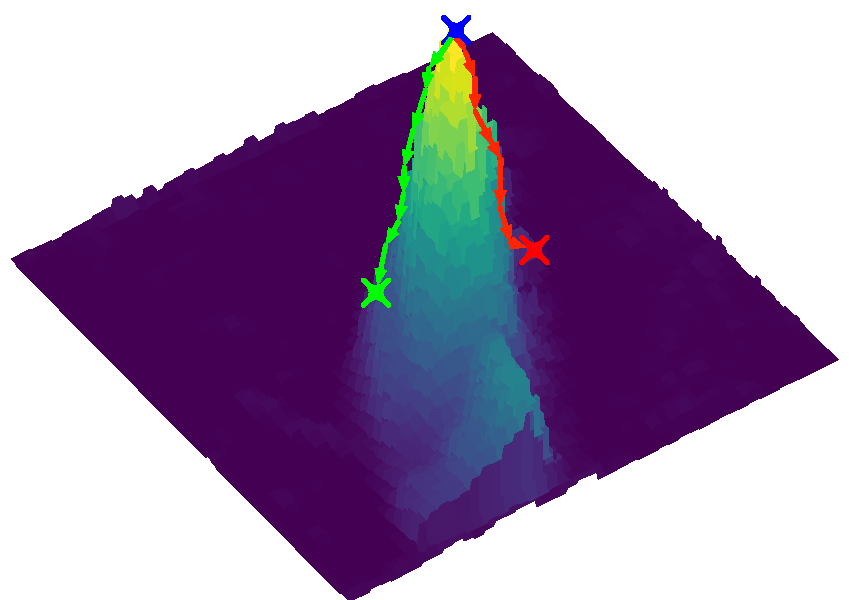
\includegraphics[width=\linewidth]{./img/scene_learning/ridge_climbing_perp.pdf}
        \subcaption{}
        \label{subfig:scene-ridge-climbing-perp}
    \end{subfigure}%
    \caption{3D visualization of the distribution of the first topic in \ref{fig:scene-topics} and ridge climbing illustration on it: along the dominant topic direction (\subref{subfig:scene-ridge-climbing}) and its perpendicular direction (\subref{subfig:scene-ridge-climbing-perp}). Blue cross indicates the starting point, red and green point indicates the end point.}
    \label{fig:scene-ridge-clibming}
\end{figure}
    % Automatic entry/exit point learning is rarely addressed in current literature. \cite{makris2005learning} proposed a Mixture of Gaussian (MOG) methods to cluster start and end point of trajectories, however, this method is quite sensitive to noises. \cite{zhao2013counting} proposed a more robust ridge climbing method, given the HDP result above. Here we proposed an improvement of it based on sampling, adapting to more complicated videos.
    \begin{figure}
\centering
    \begin{subfigure}{0.26\linewidth}
        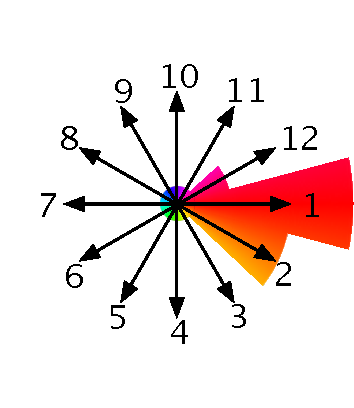
\includegraphics[width=\linewidth]{./img/scene_learning/grid_distribution.pdf}
        \subcaption{}
        \label{subfig:scene-grid-dist}
    \end{subfigure}
    \begin{subfigure}{0.35\linewidth}
        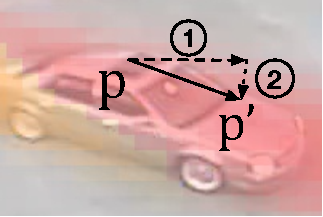
\includegraphics[width=\linewidth]{./img/scene_learning/step.pdf}
        \subcaption{}
        \label{subfig:scene-step}
    \end{subfigure}
    \begin{subfigure}{0.35\linewidth}
        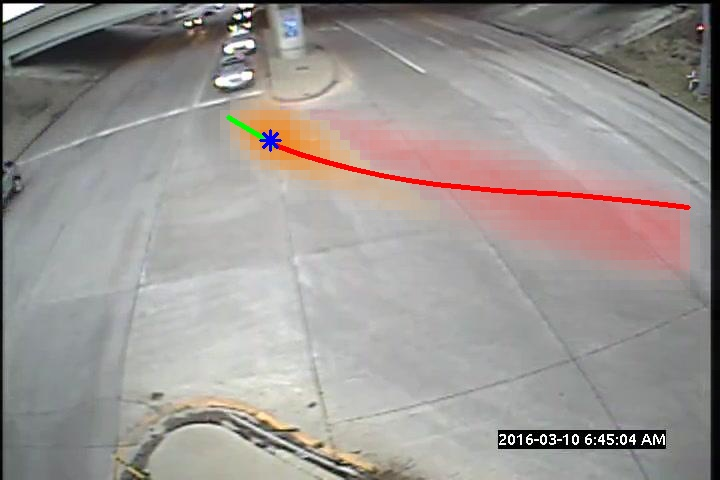
\includegraphics[width=\linewidth]{./img/scene_learning/single_ridge-1.jpg}
        \subcaption{}
        \label{subfig:scene-single-ridge}
    \end{subfigure}%
    \caption{(\subref{subfig:scene-grid-dist}) is an example of the topic distribution on one grid $i$, where the radius of each circle sector indicates $\bm{\phi}_i= [\phi_i^{1}, \phi_i^{2}, \dots, \phi_i^{D}]$. (\subref{subfig:scene-step}) shows the move-adjust step of each iteration. (\subref{subfig:scene-single-ridge}) is an extracted ridge starting from the highest density grid, where the blue star indicates the highest density grid, green and red line indicates ridges to the start/end point separately.}
    \label{fig:scene-step}
\end{figure}

    We propose a two-step movement in each iteration: first, we take a step, the step size is the normalized mean density on all the direction in its neighborhood; second, we adjust the step by moving toward higher density area. 
    The above steps are illustrated in Figure \ref{subfig:scene-step}, represented in dash lines, the final step is in solid line. 
    Mathematically, the two-step movement from $\bm{p}$ to $\bm{p^*}$ is represented as:
    \begin{align}
        \bm{p}' =&\bm{p} + \frac{\bm{v}}{||\bm{v}||_2}, \quad
        & \bm{v} = & \frac{\sum_{i=1}^n{ f(\bm{\omega})\cdot\bm{\phi}_i}}{{\sum_{i=1}^n{\varphi_i}}}, \label{eq:move}\\
        \bm{p}^* =& \bm{p}' + \alpha\cdot \bm{m}, \quad
        & \bm{m} = &\frac{\sum_{j=1}^n{\varphi_j\times(\bm{p}_i-\bm{p}')}}{\sum_{j=1}^n{\varphi_j}}.\label{eq:adjust}
    \end{align}
    We define a $2\times D$ matrix $\bm{\omega} = [\bm{\omega}_1, \bm{\omega}_2, \dots, \bm{\omega}_D]$, each column $\bm{\omega}_{d}$ is the unit vector along the quantized direction $d$.
    $\bm{v}$ and $\bm{m}$ correspond to the move and adjust step, separately. 
    For the move step \ref{eq:move}, $f(\bm{\omega})$ defines movement of each $\bm{\omega}_d$ wrt. a desired moving direction, which is the same size with $\bm{\omega}$. 
    Here we choose a neighborhood with $n$ grids around $\bm{p}$, and $\bm{p}_{i}$ is the coordinate of the $i$th grid in the neighborhood. 
    Therefore, $f(\bm{\omega})\cdot\bm{\phi}_i$ is the mean direction weighted by densities on each direction. 
    However, the moving step may not follow the elongated shape of the topic due to the uncertainty introduced by the quantized direction, where an example is given in \ref{subfig:scene-step}. 
    To deal with it, we make an adjustment on the result of the move step \ref{eq:adjust}, once reaching a lower density area, $\bm{m}$ will pull the point back to the higher-density area and make the final step (solid arrow in Figure \ref{subfig:scene-step}) better follow the shape of the topic, as illustrated in step 2 in Figure \ref{subfig:scene-step}.
    Note that in the adjust step, we compute a new neighborhood around the result of the move step.
    Intuitively, if we reach a grid that has significantly different densities, we tend to take a smaller step in case the step size is too large to follow the density surface. 
    On the contrary, if the first step reaches a grid with a roughly uniform distribution around, $\bm{m}$ tends to be a zero vector and has no effect on the final step.
    Due to the normalization term, $\bm{v}$ and $\bm{m}$ has magnitude at most $1$ in (\ref{eq:move}) and (\ref{eq:adjust}). 
    To make sure the adjust step does not cancel out the movement of step one, we normalize $\bm{v}$ into a unit vector. By setting $\alpha\in(0,1)$, it has a fixed impact on the final step. We observe that $\alpha\in[0.1,0.2]$ gives a reasonable result.

    Figure \ref{subfig:scene-ridge-climbing} gives an visual illustration of the ridge climbing process along the dominate direction, and Figure \ref{subfig:scene-single-ridge} shows the resulting ridge. The process starts from the grid with the highest $\varphi$, indicated by the blue cross, along the dominate direction, in this case, direction 1. 
    The red line is the path to the end point of the ridge, with $f(\bm{\omega}) = \bm{\omega}$; while the green line reaches the start point, obtained by setting $f(\bm{\omega}) = -\bm{\omega}$. So far the results are similar with those in \cite{zhao2013counting}.

    \begin{figure}
\centering
    % \begin{minipage}{0.48\linewidth}
    \begin{subfigure}{0.32\linewidth}
        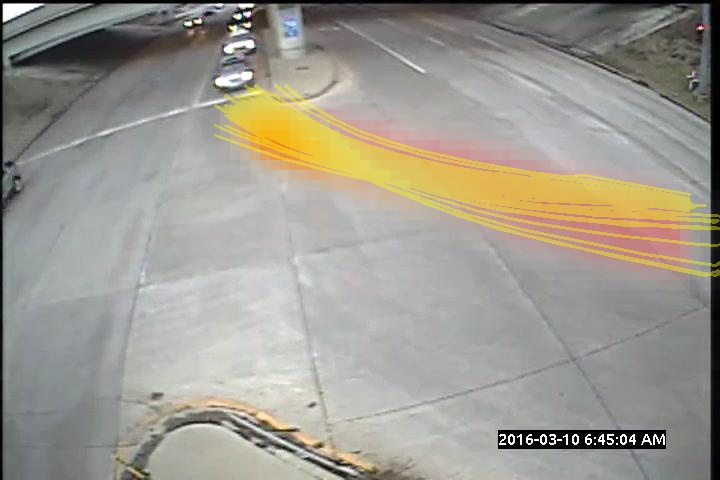
\includegraphics[width=\linewidth]{./img/scene_learning/ridges-1.jpg}
        \subcaption{}
        \label{subfig:scene-ridges}
    \end{subfigure}
    \begin{subfigure}{0.32\linewidth}
        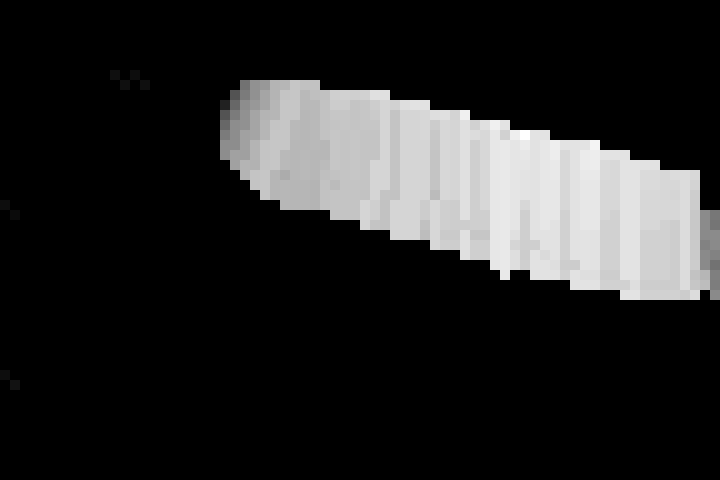
\includegraphics[width=\linewidth]{img/scene_learning/perp_width-1.png}
        \subcaption{}
        \label{subfig:scene-perp-width}
    \end{subfigure}
    \begin{subfigure}{0.32\linewidth}
        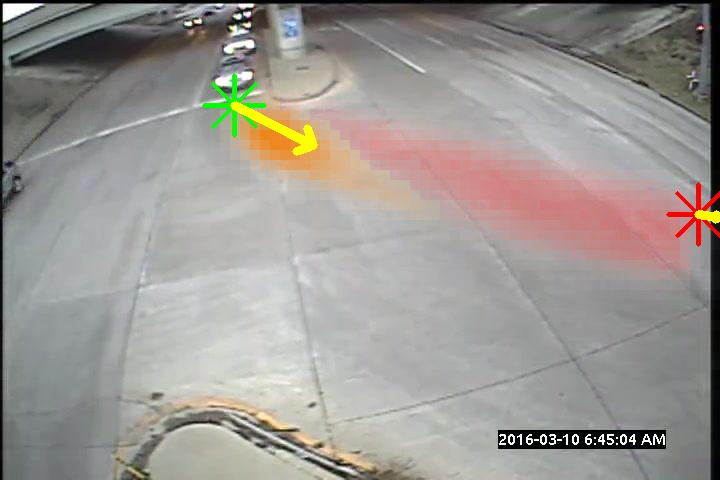
\includegraphics[width=\linewidth]{./img/scene_learning/res/middle/middle-1.jpg}
        \subcaption{}
        \label{subfig:scene-entry-exit}
    \end{subfigure}%
    \caption{(\subref{subfig:scene-ridges}): multiple ridges learned from local maximal grid. (\subref{subfig:scene-perp-width}): perpendicular width, where lighter intensity indicates a larger width. (\subref{subfig:scene-entry-exit}): extracted entry/exit hotspots indicates by the green and red star. And the yellow arrow shows their direction.}
    \label{fig:scene-ridge-res}
    % \end{minipage}
\end{figure}

% add a connection: the ridge is a single line, cannot capture the actual stripes traveled by vehicles and the dynamics of the changes in the stripe sizes. 
\subsection{Topic Extent Learning}
    Intuitively, the high-density grids indicate an active region when objects are more likely to move.
    A single ridge is not descriptive enough, especially for wide motion regions. 
    We propose two variations of the above procedure.
    First, instead of starting from the grid with global maximal $\varphi$, we start with multiple grids with local maximal $\varphi$ in its neighborhood. 
    The yellow lines in Figure \ref{subfig:scene-ridges} show the ridges extracted by the above procedure, where they roughly cover the high-density area. 
    Second, we define a \emph{perpendicular width} as the extent of the high density grids that perpendicular to the dominate direction. To obtain it, we climb the density surface along the direction perpendicular to the dominate direction $d^*_i$of the current grid $i$, demonstrated in Figure \ref{subfig:scene-ridge-climbing-perp}.
    $f(\bm{\omega})$ is obtained by rotating each unit vector $\bm{\omega}_{d}$ by 90 degrees clockwise ($f_1(\bm{\omega})$) and counterclockwise ($f_2(\bm{\omega})$). In other words, 
    \begin{align*}
        f_1(\bm{\omega}) = \left[\begin{array}{cc} 0 & -1\\ 1 & 0\end{array}\right]\cdot\bm{\omega},\quad
        f_2(\bm{\omega}) = \left[\begin{array}{cc} 0 & 1\\ -1 & 0\end{array}\right]\cdot\bm{\omega}.
    \end{align*}
    \subref{subfig:scene-perp-width} shows the learned perpendicular width of the same topic, where the lighter color indicates a larger width. The ridges and the perpendicular width together define the active resgion of a topic, giving size, location and direction of the belonging objects.
    % Adjusting the neighborhood size may result in ridges with different densities and extensions. Using a finer quantization of visual words on 12 directions makes it possible to trace the ridges in arbitrary directions.


\subsection{Entry Exit Hotspots Extraction}
\label{subsec:hdp-entry-exit}
Compared with a single ridge, ridges start from multiple locations and better indicate the start and end of motions due to their larger coverage.  The density of extracted ridges gives a nice interpretation of the area and it is unlikely for vehicles to go beyond the topic area. 
For a set of ridges $\{\bm{l}_1, \bm{l}_2, \dots, \bm{l}_m\}$, 
each of $\bm{l}_i$ is a sequence of grid coordicates $\bm{l}_i=\{\bm{p}_i^1, \bm{p}_i^2, \dots, \bm{p}_i^{s_i}\}$, 
where $s_i$ is the length of ridge $\bm{l}_i$. 
We take the first and last point of each ridge, call them \emph{candidates} of the entry/exit hotspot. Formally defined as 
$$\mathbf{Z}_\text{entry} = \{\bm{p}_1^1, \bm{p}_2^1, \dots, \bm{p}_m^1\},\; \quad
\mathbf{Z}_\text{exit} = \{\bm{p}_1^{s_1}, \bm{p}_1^{s_2}, \dots, \bm{p}_1^{s_m}\}.$$
Similarly, each has its own direction: 
\begin{align*}
\mathbf{V}_\text{entry} =& \{\bm{p}_1^2 -\bm{p}_1^1, \dots, \bm{p}_m^2-\bm{p}_m^1\},\\
\mathbf{V}_\text{exit} = &\{\bm{p}_1^{s_1}-\bm{p}_1^{s_1-1}, \dots, \bm{p}_{m}^{s_m}-\bm{p}_{m}^{s_m-1}\}.
\end{align*}
Averaging over the coordinations and directions of candidates, we have a mean location and direction for each entry and exit hotspot: 
\begin{align}
\bm{p}_{entry} = \frac{\sum_{i=1}^m{\bm{p_i^1}}}{m},\;\quad&\bm{v}_{entry} = \frac{\sum_{i=1}^m{\bm{p_i^2}-\bm{p_i^1}}}{m},\\
\bm{p}_{exit} = \frac{\sum_{i=1}^m{\bm{p_i^{s_m}}}}{m},\;\quad&\bm{v}_{exit} = \frac{\sum_{i=1}^m{\bm{p_i^{s_m}}-\bm{p_i^{s_m-1}}}}{m}.
\end{align}
\ref{subfig:scene-entry-exit} gives an visual result of the above process, 
where the green and red star corresponds to $\bm{p}_{entry}$ and $\bm{p}_{exit}$, the yellow arrow shoes their directions $\bm{v}_{entry}$ and $\bm{v}_{exit}$.
% It is worth noting that the ellipses do not indicate the size of the entry/exit area, but the area most source/sink points fall in.
Although entry/exit hotspots are also able to be obtained by fitting the start/end points of trajectories, they are less reliable than statistics learned from lower-level representation, since we are working on a tracking framework.

% \subsection{Road Skeleton}
% Next, we apply the Adaptive Multi-Kernel-based Shrinkage (AMKS) method \cite{xu2015unsupervised} to the extracted ridges, which is originally proposed for trajectory clustering. Roughly speaking, it is a clustering method along a certain direction. In this case, it is specific to the moving direction of the motions. In every iteration, each ridge moves toward the center. Ideally, after convergence, all the ridges will move to one centerline. Then the overlapped line is extracted as the final road skeleton. Before clustering, the overlapped ridges are filtered to reduce the computation overhead. The blue line in the right image in \ref{fig:scene} gives an example, where the dot at the right end indicates the sink. 
% \textcolor{red}{may discard it if not used by the tracker.}